\documentclass[sigconf]{acmart}

\usepackage{booktabs} % For formal tables
\usepackage{tabularx}
\usepackage{upgreek}

% Copyright
% \setcopyright{none}
\setcopyright{acmcopyright}
%\setcopyright{acmlicensed}
% \setcopyright{rightsretained}
%\setcopyright{usgov}
%\setcopyright{usgovmixed}
%\setcopyright{cagov}
%\setcopyright{cagovmixed}

\acmConference[Foundations of Software Science]{NC State}{Fall 2018}{Computer Science}


\begin{document}
\title{Coverage Is Not Strongly Correlated with Test Suite Effectiveness}
\subtitle{ICSE 2014}


\author{Fahmid Morshed Fahid}
\affiliation{%
  \institution{North Carolina State University}
}
\email{ffahid@ncsu.edu}

\begin{abstract}
The effectiveness of a test suite is often measured with coverage and used as a proxy for its ability to detect faults. But unfortunately, previous studies failed to reach a consensus about the nature and strength of such relationship, mostly due to small or synthetic programs, confounding influence of test suite size and using impractical adequate suites.\\
To study the relationship between test suite size, coverage and effectiveness, Inozemtseva et al.~\cite{inozemtseva2014coverage} used large Java programs with 31000 test suits for five systems consisting of up to 724,000 lines of source code. They measured the statement coverage, dicision coverage and modified condition coverage of these suites and used mutattion testing to evaluate their fault detection effectiveness.\\
Inozemtseva et al.~\cite{inozemtseva2014coverage} found that, there is a low to moderate correlation between coverage and effectiveness when the number of test cases in the suite is controlled for. Also, stronger forms of coverage do not provide greater insight into the effectiveness of the suite. Their results suggest that, coverage, while useful for identifying under-tested parts of a program, should not be used as a quality target because it is not a good indicator of test suite effectiveness.



\end{abstract}

\keywords{Universal Defect Prediction Model, Rank Transformation, Bug}

\maketitle
\section{Introduction}
Testing is an important part of producing high quality software, but its effectiveness depends on the quality of the Test Suite. Testing textbooks often recommend coverage as one of the metrics for measuring effectiveness of a test suite. \\% \cite{perry2007effective}. \\
But unfortunately, previous works found contradictory results. For example, Gligoric et al. \cite{gligoric2015guidelines} found that, effectiveness of each test suite using mutation testing has a Kendall's $\tau$ correlation from 0.452 to 0.757 when size of the suite is not considered and from 0.585 to 0.958 when considered. On a different experiment, Gopinath et al. \cite{gopinath2014code} found that, coverage is correlated with effectiveness across project with for all coverage types and suite size do not improve the results. \\
Due to different assumptions such as small or synthetic programs, confounding influence of test suite size and using impractical adequate suites, no consensus was found in code coverage as measure of effectiveness in a test suite. That's why, Inozemtseva et al \cite{inozemtseva2014coverage} proposed three research questions.
\begin{itemize}
    \item \textbf{RQ1:} Is The Size Of A Test Suite Correlated With Effectiveness?
    \item \textbf{RQ2:} Is The Coverage Of A Test Suite Correlated With Effectiveness When Suite Size Is Ignored?
    \item \textbf{RQ3:} Is The Coverage Of A Test Suite Correlated With Effectiveness When Suite Size Is Fixed?
\end{itemize}


\begin{table}
\begin{center}
\caption{Important characteristics of the subject programs.}
 \begin{tabular}{p{2.5cm} p{.8cm} p{.8cm} p{1.1cm} p{.8cm} p{.7cm}}
 \hline
 \textbf{Property} & \textbf{Apache POI} & \textbf{Closure} & \textbf{HSQLDB} & \textbf{JFree Chart} & \textbf{Joda Time}\\[0.5ex] 
 \hline
 Total Java SLOC & 283,845 & 724,089 & 178,018 & 125,659 & 80,462 \\ 

 Test SLOC & 68,832 & 93,528 & 18,425 & 44,297 & 51,444 \\
 
 Statement coverage & 67\% & 76\% & 27\% & 54\% & 91\%\\
 
 Decision coverage & 60\% & 77\% & 17\% & 45\% & 82\%\\
 
 MC coverage & 49\% & 67\% & 9\% & 27\% & 70\%\\ [1ex] 
 \hline
 \# mutants & 27,565 & 30,779 & 50,302 & 29,699 & 9,552\\
 \# detected mutants & 17,835 & 27,325 & 50,125 & 23,585 & 8,483\\
 Equivalent mutants & 35\% & 11\% & 0.4\% & 21\% & 11\%\\[1ex]
 \hline
\end{tabular}
\end{center}
\end{table}

\section{Methodology}
\begin{figure*}
\vspace{10pt}
\includegraphics[width=\textwidth,height=7cm]{Figures/Coverage_result.JPG}
\caption{Normalized effectiveness scores (left axis) plotted against coverage (bottom axis) for all subjects. Rows show the results for one suite size; columns show the results for one project.}
\label{f1}
\end{figure*}

\subsection{Terminology}
\begin{itemize}
    \item \textbf{Master suite:} Test suite written by developers of a subject program. The all other suites are strict subsets of this suite.
    \item \textbf{Mutant and Equivalent Mutant: }A mutant is a new version of the program that is created by making a small syntactic change to the original program. If resulting mutant produce the same output, it is called an equivalent mutant.
    %(i.e. negating a branch condition, or removing a method call etc.).
\end{itemize}

\subsection{Subject Program}
They have used a number of criteria to select these projects. 
\begin{itemize}
    \item Large projects on Java (on the order of 100,000 SLOC), actively developed.%novelty and generalizability
    \item Large number of test methods (on the order of 1,000). %generate reasonably sized random test suites
    \item Ant as a build system and JUnit as a test harness, to automate data collection.
\end{itemize}

\subsection{Generate Faulty Program}
Inozemtseva et al. \cite{inozemtseva2014coverage} used the open source tool \textbf{PIT} \cite{coles2016pit} to generate large number of mutants and run the program’s test suite on each one. If the test suite fails when it is run on a given mutant, the suite is said to kill that mutant, else it is equivalent. A test suite’s mutant coverage is the fraction of mutants that it kills.

\subsection{Generate Test Suite}
%reflection API
For each program, they have identified all of the test methods in the master suite. Then generated new test suites of fixed size by randomly selecting a subset of these methods without replacement. They made 1,000 suites for the following sizes: 3 methods, 10 methods, 30 methods, 100 methods, and so on. This resulted in a total of 31,000 test suites.

\subsection{Measuring Coverage}
Inozemtseva et al. used the open source tool \textbf{CodeCover} \cite{scheller2008codecover} to measure coverage. They used two effectiveness measurements in this study: normalized and non-normalized. The normalized effectiveness measurement is the number of mutants a test suite detected divided by the number of non-equivalent mutants it covers. For non-normalized results, see \cite{inozemtseva2014coverage}

\section{Case Study Results}
\begin{figure*}
\vspace{10pt}
\includegraphics[width=\textwidth,height=8cm]{Figures/Coverage_result.JPG}
\caption{Normalized effectiveness scores (left axis) plotted against coverage (bottom axis) for all subjects. Rows show the results for one suite size; columns show the results for one project. N/A indicates that the project did not have enough test cases to fill in that frame.}
\label{f1}
\end{figure*}

\textbf{RQ1: Can a context-aware rank transformation provide predictive power comparable to the power of log transformation?}\\
rank transformations to the models built using log transformations. Table 1. presents the mean values of the six performance measures of both log and rank transformations, and the corresponding p-values of Wilcoxon rank sum test. The
results show the difference between the two transformations is small (i.e., less than 0.10). They concluded that rank transformation achieves comparable performance to log transformation. It is reasonable to use the proposed rank transformation method to build universal defect prediction models.\\
\textbf{RQ2: What is the performance of the universal defect
prediction model?}\\
and the AUC value. Hence, the context factors are good predictors for building a universal defect prediction model.\\
\textbf{RQ3: What is the performance of the universal defect prediction model on external projects?}\\
ble predictive power.


\begin{table}
\begin{center}
\label{tab:coverageTable}
\caption{The Kendall $\tau$ and Pearson correlations between different types of coverage for all suites from all projects.}
 \begin{tabular}{c c c} 
 \hline
 \textbf{Coverage Types} & \textbf{Kendall's }$\uptau$ & \textbf{Pearson's r}\\ [0.5ex] 
 \hline
 Statement/Decision & 0.92 & 0.99 \\ 
 
 Decision/MCC & 0.91 & 0.98 \\
 
 Statement/MCC & 0.92 & 0.97 \\
 \hline
\end{tabular}
\end{center}
\end{table}
\section{Conclusion}
In future, their plan is to evaluate the feasibility of the universal
model for commercial projects. They have also thought about making a plugin for a version control system or IDE.
%\section{Introduction}
In this study, the authors propose a context-aware rank transformation to address the variations in the distribution of predictors before fitting them to the universal defect prediction model. They used 21 code metrics, five process metrics, and six context factors as predictors (i.e., programming language, issue tracking, the total lines of code, the total number of files, the total number of commits, and the total number of developers). The context-aware approach stratifies the entire set of projects by context factors, and clusters the
projects with similar distribution of predictors. They applied every tenth quantile of predictors on each cluster to formulate ranking functions. After transformation, the predictors from different projects have exactly the same scales. The universal model was then built based on the transformed predictors.\\
They applied their approach on 1,398 open source projects hosted on SourceForge and GoogleCode. They examined the generalizability of the universal model
by applying it on five external projects also.\\
They claimed that their main contributions are:

\begin{enumerate}
\bf\item Context-aware rank transformation

\bf\item Context factors as predictors of the universal model
\end{enumerate}


\begin{table}
\begin{center}
\caption{Important characteristics of the subject programs.}
 \begin{tabular}{|p{2.5cm}| p{1cm}| p{1cm}| p{1.2cm}| p{1cm}| p{1cm}|}
 \hline
 \textbf{Property} & \textbf{Apache POI} & \textbf{Closure} & \textbf{HSQLDB} & \textbf{JFree Chart} & \textbf{Joda Time}\\[0.5ex] 
 \hline
 Total Java SLOC & 283,845 & 724,089 & 178,018 & 125,659 & 80,462 \\ 

 Test SLOC & 68,832 & 93,528 & 18,425 & 44,297 & 51,444 \\
 
 Statement coverage & 67\% & 76\% & 27\% & 54\% & 91\%\\
 
 Decision coverage & 60\% & 77\% & 17\% & 45\% & 82\%\\
 
 MC coverage & 49\% & 67\% & 9\% & 27\% & 70\%\\ [1ex] 
 \hline
 \# mutants & 27,565 & 30,779 & 50,302 & 29,699 & 9,552\\
 \# detected mutants & 17,835 & 27,325 & 50,125 & 23,585 & 8,483\\
 Equivalent mutants & 35\% & 11\% & 0.4\% & 21\% & 11\%\\[1ex]
 \hline
\end{tabular}
\end{center}
\end{table}


\section{Data Preprocessing}

It is very likely that predictors from different projects of various contexts exhibit different distribution  \cite{zhang2013does}. To overcome this challenge towards building a universal defect prediction model, they proposed a context-aware rank transformation approach, as illustrated in Figure 1.

\begin{figure*}
\vspace{10pt}
\includegraphics[width=\textwidth,height=8cm]{Coverage_result.JPG}
\caption{Normalized effectiveness scores (left axis) plotted against coverage (bottom axis) for all subjects. Rows show the results for one suite size; columns show the results for one project. N/A indicates that the project did not have enough test cases to fill in that frame.}
\label{f1}
\end{figure*}



\section{Context Factors}
They chose six context factors based on their availability to open source projects.
\begin{enumerate}
\bf\item Programming Language (PL)
\bf\item Issue Tracking (IT) 
\bf\item Total Lines of Code (TLOC)
\bf\item Total Number of Files (TNF)
\bf\item Total Number of Commits (TNC)
\bf\item Total Number of Developers (TND)
\end{enumerate}
They stratified the entire set of projects based on the aforementioned six context factors. They got 5,2,4,4,4, and 4 groups, respectively. In total, They obtained 2560 (i.e.,$ 5 $ x $2 $ x $4$ x $4$ x $4$ x $4$) non-overlapped groups.


\section{Clustering Similar Projects}
To derive more accurate quantiles of a particular metric, They grouped the projects with the similar distribution of the metric. Two distributions are similar if their difference is neither statistically significant nor significantly large. For each metric m, the clusters of projects with the similar distribution of metric m are obtained using an algorithm. It has two major steps:-

\begin{enumerate}
\item Comparing the Distribution of Metrics - Mann-Whitney U test was used
\item Quantifying the Difference between Distributions - Cliff's $\delta$ was used
\end{enumerate}

\section{Obtaining Ranking Functions}
\begin{table}
\begin{center}
\label{tab:coverageTable}
\caption{The Kendall $\tau$ and Pearson correlations between different types of coverage for all suites from all projects.}
 \begin{tabular}{c c c} 
 \hline
 \textbf{Coverage Types} & \textbf{Kendall's }$\uptau$ & \textbf{Pearson's r}\\ [0.5ex] 
 \hline
 Statement/Decision & 0.92 & 0.99 \\ 
 
 Decision/MCC & 0.91 & 0.98 \\
 
 Statement/MCC & 0.92 & 0.97 \\
 \hline
\end{tabular}
\end{center}
\end{table}


The ranking function transforms the raw metric values to relatively predefined values (i.e., ranging from one to ten). The researchers  used the quantiles of metric values to formulate our ranking functions. For example, if every tenth quantile for a metric m1 in cluster Cl is: $11, 22, 33, 44, 55, 66, 77, 88,$
and $99$ respectively. Then the value 27 of metric m1 will be converted to 3 if the corresponding project belongs to cluster Cl. This is because the value 27 is greater than 22 (i.e., the 20$\%$ quantile) and less than 33 (i.e., the 30$\%$ quantile)

\section{Building a Universal Defect Prediction Model}
They applied Naive Bayes as the modelling technique in their experiments. Before transforming a metric $m_{i}$ for project $p_{j}$ , we identify context factors of project $p_{j}$ and formulate a vector like $< m_{i}, C++, useIT, moreT LOC, lessT NF, lessT NC, lessT ND >$.  In order to locate the ranking functions, they compared the vector of project $p_{j}$ to the vectors of all clusters to determine which cluster project $p_{j}$ belongs to.

\section{Case Study Results}
\textbf{RQ1: Can a context-aware rank transformation provide predictive power comparable to the power of log transformation?}\\
rank transformations to the models built using log transformations. Table 1. presents the mean values of the six performance measures of both log and rank transformations, and the corresponding p-values of Wilcoxon rank sum test. The
results show the difference between the two transformations is small (i.e., less than 0.10). They concluded that rank transformation achieves comparable performance to log transformation. It is reasonable to use the proposed rank transformation method to build universal defect prediction models.\\
\textbf{RQ2: What is the performance of the universal defect
prediction model?}\\
and the AUC value. Hence, the context factors are good predictors for building a universal defect prediction model.\\
\textbf{RQ3: What is the performance of the universal defect prediction model on external projects?}\\
ble predictive power.


\begin{table}
\begin{center}
\caption{The performance measures for the universal models built using CM , CPM and CPMC}
 \begin{tabular}{|c c c c |} 
 \hline
 \textbf{Measures} & \textbf{CM} & \textbf{CPM} & \textbf{CPMC}\\ [0.5ex] 
 \hline
 prec & 0.36 & 0.38 & 0.40 \\ 
 \hline
 pd & 0.91 & 0.83 & 0.86 \\
 \hline
 fpr & 0.87 & 0.76 & 0.70 \\
 \hline
 F-measure & 0.51 & 0.51 & 0.55\\
 \hline
 g-measure & 0.23 & 0.36 & 0.42\\
 \hline
 AUC & 0.58 & 0.60 & 0.65\\ [1ex] 
 \hline
\end{tabular}
\end{center}
\end{table}

%\section{Threats to validity}
%The main threats that they mentioned on their paper is due to data cleaning. They neglected a large no. of projects with negligible fix-inducing or non-fixing commits

\section{Conclusion}
In future, their plan is to evaluate the feasibility of the universal
model for commercial projects. They have also thought about making a plugin for a version control system or IDE.







\bibliographystyle{ACM-Reference-Format}
\bibliography{bibliography}

\end{document}